\documentclass[10pt]{scrartcl}

\usepackage[utf8]{inputenc}
\usepackage{tabularx}
\usepackage[ngerman]{babel}
\usepackage[automark]{scrpage2}
\usepackage{amsmath,amssymb,amstext}
%\usepackage{mathtools}
\usepackage[]{color}
\usepackage[]{enumerate}
\usepackage{graphicx}
\usepackage{lastpage}
\usepackage[perpage,para,symbol*]{footmisc}
\usepackage{listings} 
\usepackage[pdfborder={0 0 0},colorlinks=false]{hyperref}
\usepackage[numbers,square]{natbib}
\usepackage{color}
\usepackage{colortbl}
\usepackage{listings}
\usepackage{a4wide}
\usepackage{xspace}
\usepackage{listings}
\usepackage{hyperref}
\usepackage{epstopdf}
\usepackage{amsmath}
\usepackage[colorinlistoftodos,textsize=small,textwidth=2cm,shadow,bordercolor=black,backgroundcolor={red!100!green!33},linecolor=black]{todonotes}

\lstset{numbers=left, numberstyle=\tiny, numbersep=5pt, breaklines=true, showstringspaces=false} 

%changehere
\def\titletext{TT2 Problemstellung 1 : Zusammenfassung}
\def\titletextshort{Problemstellung 1}
\author{Carsten Noetzel}

\title{\titletext}

%changehere Datum der Übung
\date{12.05.2012}

\pagestyle{scrheadings}
%changehere
\ihead{TT2, Neitzke}
\ifoot{Generiert am:\\ \today}

\cfoot{Carsten Noetzel}


\ohead[]{\titletextshort}
\ofoot[]{{\thepage} / \pageref{LastPage}}

\setlength{\parindent}{0.0in}
\setlength{\parskip}{0.1in}

\begin{document}
\maketitle

\setcounter{tocdepth}{3}
\tableofcontents
\listoffigures
%\lstlistoflistings

\section{Einführung}
\subsection{Lernsituationen}
\subsubsection{Überwachtes Lernen - \glqq supervised learning\grqq}
Ein Lehrer sagt was das richtige Ergebnis gewesen wäre.
\subsubsection{Unüberwachtes Lernen - \glqq unsupervised learning\grqq}
Das System bemerkt selbst, dass es unterschiedliche Eingangsklassen gibt.

\subsubsection{(Ver-)Bestärkendes Lernen - \glqq reinforcement learning\grqq}
Der Lehrer (Leben/Umgebung) belohnt oder bestraft.

\section{Reinforcement Learning}
\subsection{Einführung}
Beim Reinforcement Learning wird der Agent in einer Umgebung platziert, in der er agiert und aus einer Reihe von \textbf{Belohnungen/ Bestrafungen} lernt. Anders als beim überwachten Lernen, werden dem Agenten \textbf{keine Trainingsbeispiele} vorgegeben, der Agent lernt demnach nur aus seiner eigenen Erfahrung. In vielen Anwendungsbereichen ist es gar nicht möglich Trainingsbeispiele bereitzustellen, anhand derer ein Agent lernen kann (z.B. Schach), somit ist man gezwungen eine andere Form des Lernens anzuwenden.\\
Das Reinforcement (die Belohnung/Bestrafung) kann dabei entweder \textbf{direkt nach einer Aktion} oder \textbf{erst am Ende} erfolgen, in diesem Fall muss der Agent dann prüfen, welche der Aktionen am Wahrscheinlichsten die Ursache für das Ergebnis ist.

\begin{figure}[htbp]
	\centering	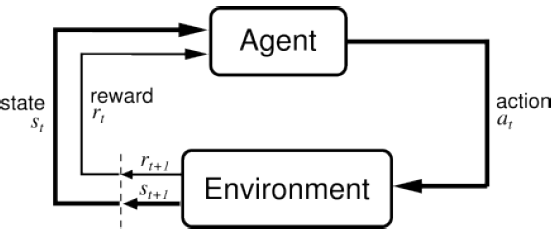
\includegraphics[width=0.5\textwidth]{Bilder/Agent.png}
	\caption{Agent in seiner Umgebung}
	\label{fig:Agent}
\end{figure}

Der Agent befindet sich zu jedem Zeitpunkt  einem Zustand $s_{t}$ und wählt eine Aktion $a_{t}$ aus, die in der Umgebung ausgeführt wird. Der Agent gelangt daraufhin in den Folgezustand $s_{(t+1)}$ und erhält die Belohnung/Bestrafung $r_{(t+1)}$ von der Umgebung. Belohnung/Bestrafung und Folgezustand sind demnach Phänomene der Umgebung, die vom Agenten beobachtet werden (Modell der Umgebung).\\
Die \textbf{Umgebung} ist im Allgemeinen \textbf{nicht deterministisch} (die gleichen Aktionen im gleichen Zustand, können zu unterschiedlichen Folgezuständen führen) \textbf{aber stationär} (Wahrscheinlichkeiten für Folgezustände bei gegebener Aktion ändern sich nicht im Laufe der Zeit).

\subsection{Policy - Strategie}
Welche Aktion abhängig vom Zustand wählen?

\subsubsection{stochastische Strategie}
Für einen Zeitpunkt t gibt es eine Wahrscheinlichkeit $\pi_{t}(s,a)$ dafür, dass a die gewählte Aktion $a_{t}$ sein wird falls $s$ der aktuell vorliegende Zustand $s_{t}$ sein sollte. Ziel des Agenten ist es seine Belohnungen über die Gesamtlaufzeit zu maximieren, also die optimale Strategie $\pi^{*}$ zu lernen.

\subsubsection{deterministische Strategie}
Die deterministische Strategie mappt Zustände direkt auf Aktionen $\pi: S \rightarrow A$, wobei $S$ die Menge der Zustände und $A$ die Menge der Aktionen ist, mit $A(s)$ als mögliche Aktionen im Zustand $s$. (siehe Reflex Agent)

\subsubsection{$\varepsilon$-greedy}
Meistens wird die Aktion mit dem höchsten erwarteten Reward gewählt (greediest action), mit einer Wahrscheinlichkeit $\varepsilon$ jedoch zufällig eine andere (unabhängig vom erwarteten Reward).

Wahrscheinlichkeitsvektor über die möglichen Aktionen in einem Zustand: $\vec x = (x_1, x_2, x_3, ..., x_n)$ mit $n$ als der Anzahl möglicher Aktionen und $x_i$ der Wahrscheinlichkeit, Aktion $i$ zu wählen.

\[
x_i=\begin{cases}
  (1-\varepsilon) + (\varepsilon/n),  & \text{wenn }Q\text{ von }i\text{ am höchsten in }\vec x\text{ ist.}\\
  \varepsilon/n, & \text{sonst.}
\end{cases}
\]

\subsubsection{$\varepsilon$-soft}
Meistens wird die Aktion mit dem höchsten erwarteten Reward gewählt, mit einer Wahrscheinlichkeit $1-\varepsilon$ jedoch zufällig eine andere (unabhängig vom erwarteten Reward).

\subsubsection{softmax}
Jede Aktion wird anhand ihres zu erwarteten Rewards gewichtet. Es wird zufällig eine Aktion ausgewählt, allerdings mit Betrachtung des Gewichts, sodass die Aktion, die den schlechtesten Reward bringt auch am seltensten gewählt wird. 

Dies unterbindet den Nachteil von $\varepsilon$-greedy bzw. $\varepsilon$-soft, dass, abgesehen von der besten Aktion, immer zufällig irgendeine Aktion gewählt wird. Bei diesen beiden Ansätzen könnte es sein, dass bei der zufälligen Wahl der Aktion immer die schlechteste gewählt wird.

\subsection{Belohnungen}
\subsubsection{episodische Aufgaben}
Der Return ist die Summe der \textbf{Rewards ab dem Zeitpunkt $t$}, bei dem $T$ ein abschließender Schritt wäre  $R_{t}= r_{(t+1)}+ r_{(t+2)}+ r_{(t+3)}+ ... +r_{T}$. Führt der Agent \textbf{episodische Aufgaben} aus, enden diese jeweils mit einem abschließenden Schritt. Hierbei wird zwischen der Menge der nicht-terminalen Zustände $S$ und der Menge aller Zustände $S^{+}$ unterschieden.

\subsubsection{kontinuierliche Aufgaben}
Sind fortdauernde Aufgaben. Da nicht endende Aufgaben zu einer unendlich hohen Belohnung führen würden, muss der \textbf{Reward abgeschwächt} werden (\textbf{discounting}). Die Abschwächung erfolgt hierbei über eine Discount-Rate $0 \leq \gamma  \leq 1$ die die Gesamtbelohnung begrenzt. Für den Reward ergibt sich somit: 
\begin{equation}
R_{t}= r_{(t+1)}+ \gamma*r_{(t+2)}+ \gamma^2*r_{(t+3})+ ... = \sum_{k=0}^\infty \gamma^{k}* r_{(t+k+1)}
\end{equation}

\subsection{Agenten-Designs}
\subsubsection{Utility Based Agent}
Der Agent lernt eine \glqq Utility Function\grqq\xspace und nutzt diese um einen Zustand zu bewerten. Diese wird genutzt um auf Basis des aktuellen Zustands eine Aktion auszuwählen, die den größten Nutzen bringt. Hierzu benötigt der Agent aber ein Modell der Umwelt, um die Folgezustände der Aktionen bestimmen zu können.

\subsubsection{Q-Learning}
Diese Form von Agenten lernt eine \glqq Action-Utility Function\grqq\xspace, welche den erwarteten Nutzen einer Aktion in einem bestimmten Zustand bestimmt. Da die Aktionen verglichen werden ohne ihr genaues Ergebnis zu kennen, benötigt der Agent kein Modell der Umwelt. Dies führt dazu, dass der Agent nicht in die Zukunft blicken kann, was ggfs. Auswirkungen auf die Lernfähigkeit des Agenten hat.

\subsubsection{Reflex Agent}
Der Agent lernt eine Strategie, welche Zustände direkt auf Aktionen mapt.

\subsection{Arten}
\subsubsection{Passive Learning}
Hierbei ist die Strategie des Agenten festgelegt und seine Aufgabe ist es des Nutzen der Zustände zu lernen. Dies kann auch das Erlernen eines Modells der Umgebung beinhalten.

\subsubsection{Active Learning}
Der Agent muss zum Nutzen einzelner Zustände auch noch lernen was zu tun ist.

\subsection{Markow Decision Process (MDP)}
\subsubsection{Definition}
Markow Entscheidungsprozesse sind ein \textbf{mathematisches Framework zur Modellierung von Entscheidungssituationen} in denen das Ergebnis teilweise zufällig ist und der Kontrolle eines Entscheiders unterliegt. MDPs werden genutzt um \textbf{Optimierungsprobleme} zu untersuchen die mittels \textbf{dynamischer Programmierung} und \textbf{Reinforcement Learning} gelöst werden.\\
\\
Ein Markow Prozess ist ein 4-Tupel $(S,A,P(.,.).R(.,.))$, wobei

\begin{itemize}
\item{$S$ eine endliche Menge von Zuständen ist}
\item{$A$ eine endliche Menge von Aktionen ist}
\item{$P_{a}(s,s') = P_{r}(s_{t+1} = s' | s_{t} = s, a_{t} = a)$ die Wahrscheinlichkeit das aus Aktion $a$ im Zustand $s$ zum Zeitpunkt $t$ der  Zustand $s'$ zum Zeitpunkt $t+1$ resultiert  (Übergangswahrscheinlichkeit durch Aktion a)}
\item{$R_{a}(s,s')$ ist der Erwartungswert für die unmittelbare Belohnung, die durch den Übergang in den Zustand $s'$ erhalten wird}
\end{itemize}

Konkret sind MDPs \textbf{zeitdiskrete stochastische Prozesse}. In jedem Zeitschritt befindet sich der Prozess in einem Zustand $s$ und der \textbf{Entscheider fällt zufällig eine Entscheidung} $a$, die im Zustand $s$ ausführbar ist. Der Prozess wechselt daraufhin in den Zustand $s'$ der dem Entscheider eine entsprechende Belohnung zurückgibt $R_{a}(s,s')$. Die Wahrscheinlichkeit, dass dabei in den Zustand $s'$ gewechselt wird ist abhängig vom aktuellen Zustand und der gewählten Aktion $a$, die durch die Zustandsübergangsfunktion $P_{a}(s,s')$ beschrieben wird. Der Zustandsübergang ist demnach unabhängig von allen vorherigen Zuständen und Aktionen. Diese Gedächtnislosigkeit wird auch als \textbf{Markow-Eigenschaft} bezeichnet. Die \textbf{Umgebung liefert alle notwendigen Informationen für zukünftige Entscheidungen}.\\
MDPs sind eine \textbf{Erweiterung der Markow-Ketten}. Bei MDPs gibt es eine Auswahl an \textbf{Aktionen} (Auswahl) und \textbf{Belohnungen} (Motivation). Wenn nur eine Aktion für jeden Zustand existiert und alle Belohnungen gleich null sind, reduziert sich der Markow-Prozess zu einer Markow-Kette.

\subsubsection{Markow Entscheidungsproblem}
Das Kernproblem von MDPs ist es eine Policy (Strategie) für den Entscheider zu finden: ein Funktion $\pi$ die die Aktion spezifiziert $\pi(s)$ die im Zustand $s$ gewählt wird. Sobald ein MDP mit einer Policy kombiniert wird, werden die Aktionen für einzelne Zustände festgelegt, was zu einem Verhalten wie in einer Marow-Kette führt. Das Ziel ist es eine Policy $\pi$ zu finden, die die Belohnungen maximiert, typischerweise ist das der abgeschwächte Reward über alle Zeitschritte.

\begin{equation}
\sum_{t=0}^\infty \gamma^t R_{at}(s_{t}, s_{t+1})
\end{equation}

Hierbei ist $\gamma$ der Discount Faktor, wobei typischerweise gilt $\gamma = \frac{1}{1+r}$ mit $r$ als Discountrate. Aufgrund der Markow-Eigenschaft, dass die Auswahl der Aktionen nur vom aktuellen Zustand abhängt, kann das Problem als Funktion beschrieben werden die nur von $s$ abhängig ist, indem man für $at= \pi(s_{t})$ einsetzt. Lösungsverfahren hierfür sind die \textbf{Policy bzw. die Value Iteration}.

\subsubsection{MDP und Reinforcement Learning}
Reinforcement Learning kann das Entscheidungsproblem lösen, ohne die Zustandsübergangsfunktionen $P_{a}(s,s')$ explizit spezifizieren zu müssen. Diese \textbf{Werte werden jedoch für die Value und Policy Iteration benötigt}.\\
Anstelle die Wahrscheinlichkeiten vorzugeben, werden diese beim Reinforcement Learning ermittelt, indem die \textbf{Simulation mehrfach neu gestartet} wird und immer zufällige Initiale Zustände gewählt werden.

\subsection{Bewertungsfunktionen}
Die Bewertungsfunktionen liefern ein \textbf{Maß für die Güte von Zuständen bzw. Aktionen unter Verfolgung einer bestimmten Strategie} und sind daher nützlich für die Auswahl von Aktionen. Die Funktionen sind dem Agenten \textbf{zunächst unbekannt} und müssen vom Agenten gelernt /geschätzt werden, sie werden auch als das Gedächtnis des Agenten bezeichnet.

\subsubsection{V-Wert}
Der V-Wert eines Zustands $s$ ist der Erwartungswert (E) der aufsummierten Belohnungen, die, ausgehend von $s$ unter einer bestimmten Strategie $\pi$ erreicht werden. Die Funktion $V^{\pi}$ heißt \textbf{Zustand-Wert-Funktion} (state-value-function) und $V^{*}$ ist die optimale V-Funktion bei optimaler Strategie $\pi^{*}$.

\begin{equation}
V^{\pi}(s)= E_{\pi} \{ \sum_{k=0}^\infty \gamma^k r_{(t+k+1)} | s_{t}=s \}
\end{equation}

\subsubsection{Q-Wert}
Der Q-Wert eines Zustands $s$ ist der Erwartungswert (E) der aufsummierten Belohnungen die, ausgehend von $s$ unter Auswahl einer bestimmten Aktion $a$ und der anschließenden Verfolgung einer Strategie $\pi$ erreicht werden. Die Funktion $Q^{\pi}$ heißt \textbf{Aktion-Wert-Funktion} (action-value-function) und $Q^{*}$ ist die optimale Q-Funktion bei optimaler Strategie $\pi^{*}$.

\begin{equation}
Q^{\pi}(s,a)= E_{\pi} \{ \sum_{k=0}^\infty \gamma^k r_{(t+k+1)} | s_{t}=s, a_{t}=a \}
\end{equation}

Da die Funktion während des Lernes unbekannt ist, basiert die Erfahrung aus Paaren von $(s,a)$ in der Form \glqq Ich war im Zustand $s$ und habe $a$ ausgeführt und bin dadurch in $s'$ gelandet\grqq\xspace. Wenn man das Q-Wert Array hat und dieses durch Erfahrungen direkt aktualisiert, nennt man das \textbf{Q-Learning}.

\section{Dynamic Programming}
\label{sec:dynamicPrograming}
\subsection{Definition}
Unter dynamischer Programmierung versteht man eine Methode zum \textbf{algorithmischen Lösen von Optimierungsproblemen}. Der Begriff wurde von Richard Bellman eingeführt, weswegen auch häufig vom \glqq Bellman Prinzip der dynamischen Programmierung gesprochen\grqq\xspace wird. \textbf{Voraussetzungen} für die dynamische Programmierung sind:

\begin{itemize}
\item{Die Menge der Zustände ist bekannt und ist endlich}
\item{Die Menge der möglichen Aktionen \{a\} ist bekannt und endlich}
\item{Belohnungen für alle Zustände bekannt}
\item{Folgezustände in Abhängigkeit von Ausgangszustand und Aktion bekannt}
\end{itemize}

\todo{Sieht das nur so aus oder kann ich mit diesem ganzen Wissen auch einen $A^*$ machen ? OS}


Dynamische Programmierung lässt sich dann erfolgreich einsetzen, wenn das Optimierungsproblem aus \textbf{vielen gleichartigen Teilproblemen} besteht und sich die optimale Lösung des Problems aus den optimalen Lösungen der Teilprobleme zusammensetzt. Hierfür werden zunächst die optimalen Lösungen der \textbf{kleinsten Teilprobleme direkt berechnet} und dann geeignet zu einer Lösung eines \textbf{nächstgrößeren Teilproblems zusammengesetzt}. \textbf{Teilergebnisse werden in einer Tabelle} gespeichert, um bei nachfolgenden Berechnungen gleichartiger Teilprobleme auf die Ergebnisse zurückgreifen zu können. Bei konsequentem Einsatz vermeidet die dynamische Programmierung kostspielige Rekursionen weil bekannte Teilergebnisse wiederverwendet werden.\\
Zum Einsatz kommt die dynamische Programmierung in der Regelungstheorie und verwandten Gebieten und wird dort eingesetzt um beispielsweise Gleichungen herzuleiten (Hamilton-Jacobi-Bellman-Gleichung), deren Lösung den optimalen Wert ergibt.
Dynamic Programming hat hauptsächlich einen theoretischen Stellenwert, da die Annahme der Markov-Eigenchaft
(ein vollständiges Modell der Welt) nur schwer zu erfüllen ist und die Algorithmen rechenintensiv
sind. Alle anderen Verfahren versuchen sozusagen, durch (deutlich) geringeren Rechenaufwand
diesem Idealzustand anzunähern. 

\subsubsection{Bellman-Gleichungen $\Rightarrow$ diskrete Zeit, dynamische Programmierung}
Bellman-Gleichungen sind eine \textbf{notwendige Bedingung zur Ermittlung des optimalen Wertes}  bei der dynamischen Programmierung. Ausgehend von einer \textbf{Initialen Entscheidung} werden die Werte die sich aufgrund dieser ersten Entscheidung ergeben haben festgehalten, um die Werte der \textbf{nachfolgenden Entscheidungsprobleme} zu bestimmen. Dadurch wird das große \textbf{Optimierungsproblem in kleinere, einfachere Probleme unterteilt} wie es das \textbf{Optimalitätsprinzip von Bellman} vorschreibt (eine optimale Lösung setzt sich aus den optimalen Teillösungen zusammen).\\
\\
Der Begriff Bellman-Gleichung bezieht sich normalerweise auf die dynamische Programmierung mit diskreter Zeit, wobei bei Optimierungsproblemen mit kontinuierlicher Zeit von Hamilton-Jacobi-Bellman-Gleichungen gesprochen wird.


\subsubsection{Hamilton-Jacobi-Bellman Gleichungen $\Rightarrow$ kontinuierliche  Zeit, Regelungstheorie}
HJBs sind \textbf{partielle Differentialgleichungen} zur Lösung von Optimierungsproblemen in Systemen mit \textbf{kontinuierlicher Zeit}. Die Lösung der HJB ergibt die „Value Function“, welche die optimalen Kosten für ein dynamisches System mit einer assoziierten „Cost Function“ darstellt. Lokal gelöst ist die HJB eine notwendige Bedingung für ein Optimum, wird die HJB jedoch über alle Zustände des Raums gelöst, ist sie die notwendige und hinreichende Bedingung für ein Optimum.

\subsection{Evaluation und Improvement}
\subsubsection{Policy Evaluation (Strategie-Bewertung)}
Bei der Policy Evaluation wird zunächst die „State-Value-Function“  \textbf{einer willkürlichen für die Iteration fest vorgegebenen Strategie berechnet}. Hierbei ist $\pi(s,a)$ die Wahrscheinlichkeit die Aktion $a$ im Zustand $s$ unter Strategie $\pi$ auszuwählen.

\begin{equation}
V^\pi (s) = \sum_{a} \pi(s,a) \sum_{s^{'}} P^a_{ss^{'}} [R^a_{ss^{'}} + \gamma V^\pi (s^{'})]
\end{equation}

Für eine iterative Lösung gilt folgende Updateregel: Die Initiale Approximation $V_{0}$ wir zufällig ausgesucht und jede nachfolgende Approximation erhält man über die Bellman Gleichung für $V^{\pi}$.

\begin{equation}
V_{k+1} (s) = \sum_{a} \pi(s,a) \sum_{s^{'}} P^a_{ss^{'}} [R^a_{ss^{'}} + \gamma V_{k} (s^{'})]
\end{equation}

Zur Erzeugung der Nachfolgeapproximation $V_{k+1}$ von $V_{k}$ wird in der \textbf{iterative policy evalutation} die gleiche Operation für jeden Zustand $s$ ausgeführt: dieser ersetzt den alten Wert von $s$ mit dem neuen, welcher auf Basis der Vorgänger von $s$ und der erwartetem unmittelbaren Belohnungen berechnet wurde. Diese Form der Berechnung wird \textbf{full backup} genannt, da in jeder Iteration der berechnete Wert gespeichert wird, um im nächsten Schritt den neuen Approximationswert zu berechnen.\\
\\
Algorithmisch würde es zwei Arrays geben, eines für die gespeicherten Werte $V_{k}(s)$ und eines für die neuen Werte $V_{k+1}(s)$. Dadurch können die neuen Werte nacheinander berechnet werden, ohne dass die alten Werte sich ändern. Natürlich könnte man auch auf einem Array arbeiten und die Werte \glqq in place\grqq\xspace aktualisieren, wodurch der Algorithmus schneller nach  $V^\pi$ konvergiert, da immer die aktuellsten Werte zur Berechnung verwendet werden.\\
Der Algorithmus bricht ab, wenn der Unterschied zwischen $V_{k}(s)$ und $V_{k+1}(s)$ klein genug ist.

\begin{figure}[htbp]
	\centering	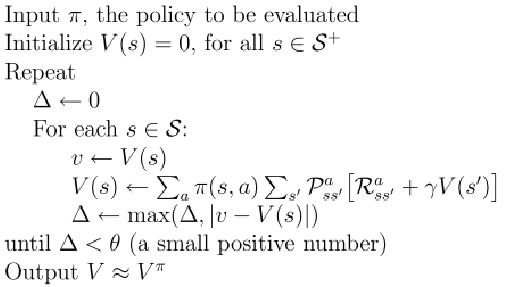
\includegraphics[width=0.5\textwidth]{Bilder/Evaluation.png}
	\caption{Algorithmus zur Evaluation einer Policy}
	\label{fig:Evaluation}
\end{figure}

\subsubsection{Policy Improvement (Strategie-Verbesserung)}
Der Grund warum wir die \glqq State-Value-Function\grqq\xspace für eine bestimmte Strategie berechnen, ist der dass sie uns helfen soll bessere Strategien zu finden. Nehmen wir an wir haben die \glqq State-Value-Function\grqq\xspace $V^{\pi}$ einer willkürlichen Strategie berechnet und möchten für einige Zustände $s$ wissen, ob wir die Strategie ändern sollten um eine Aktion zu wählen für die gilt $a \neq \pi$. Durch den \textbf{Austausch einzelner Aktionen}, kann die Strategie ggfs. verbessert werden.\\
\\  
Wenn in einem Zustand $s$ nicht der zugrundeliegenden Strategie $\pi$ gefolgt wird, sondern eine einzelne Aktion $a \neq \pi$ gewählt wird (und danach weiterhin entsprechend $\pi$ vorgegangen wird), ergibt sich folgender Wert für $s$:

\begin{align}
Q^{\pi}(s,a) &= E_{\pi} \{ r_{t+1} + \gamma V^{\pi}(s_{t+1}) | s_{t}=s, a_{t}=a \}\\
Q^{\pi}(s,a) &= \sum_{s^{'}} P^a_{ss^{'}} [R^a_{ss^{'}} + \gamma V^\pi (s^{'})]
\end{align}

Das Hauptkriterium ist, ob der durch den Austausch errechnete Wert größer oder kleiner als $V^{\pi}(s)$ ist. Wenn er größer ist, ist es besser einmal Aktion $a$ im Zustand $s$ auszuwählen und dann der Strategie $\pi$ zu folgen, anstellen $\pi$ die ganze Zeit zu verfolgen. Daraus folgend würde man erwarten, dass es immer besser ist $a$ auszuwählen, wenn man sich im Zustand $s$ befindet und dass die neue Strategie eine bessere wäre.

Die ist der Fall beim \textbf{policy improvement Theorem}, bei dem die oben genannte Annahme gilt und $\pi$ und $\pi^{'}$ beliebige deterministische Strategien sind.

\begin{equation}
Q^{\pi}(s,\pi^{'}(s)) \geq V^{\pi}(s)
\end{equation}

In diesen Fall muss die Strategie $\pi^{'}$ genauso gut oder besser als $\pi$ sein und damit eine gleich große oder bessere Belohnung für alle Zustände einholen.

\textbf{Optimale Bewertungsfunktionen}\\
Zwei Strategien können durch ihre Bewertungsfunktionen vergleichen werden. Es gilt $\pi \geq \pi^{'}$, wenn $V^{\pi}(s)\geq V^{\pi^{'}}(s)$ für alle $s \in S$.\\
\\
Die optimale Strategie verfügt über die optimale V-Funktion:  $V^{*}(s) = max_{\pi} V^{\pi}(s)$, für alle $s \in S$\\
\\
Außerdem über die optimale Q-Funktion: $Q^{*}(s,a) =  max_{\pi} Q^{\pi}(s,a)$, für alle $s \in S$, $a \in A$\\
\\
Q kann bezüglich V definiert werden: $Q^{*}(s,a) = E \{r_{t+1}+ \gamma V^{*}(s_{t+1}) | s_{t}=s ,a_{t}=a \}$

\textbf{Verallgemeinerung}\\
Gegeben sind zwei Strategien $\pi$ und $\pi^{'}$ und es gilt $Q^{\pi}(s,\pi^{'}(s)) \geq V^{\pi}(s)$ für alle $s \in S$\\
Das heißt: Es wird nur für einen Schritt nach  $\pi^{'}$ vorgegangen, danach wieder nach  $\pi$. Dann gilt für alle $s \in S$: $V^{\pi^{'}}(s) \geq V^{\pi}(s)$ !

\textbf{Berechnung einer optimalen Strategie}\\
Wiederholte Bewertung (Evaluation) einer gegebenen Strategie, dann Verbesserung (Improvement) $\Rightarrow$ Strategie-Iteration (\textbf{Policy Iteration}).

\begin{equation}
\pi_{0} \overset{E}\rightarrow V^{\pi 0} \overset{I}\rightarrow \pi_{1} \overset{E}\rightarrow V^{\pi 1} \overset{I}\rightarrow \pi_{2} \overset{E}\rightarrow \dotsb \overset{I}\rightarrow \pi^{*} \overset{E}\rightarrow V^{*}
\end{equation}

\subsection{Policy Iteration}
Bei der Policy Iteration wird eine vorhandene Strategie $\pi$ bewertet (Evaluation) und verbessert (Improvement) um eine Strategie $\pi^{'}$ zu erhalten die besser ist. Dieses Schritte werden solange wiederholt, bis die Strategie stabil  ist und sich die Werte in $\pi(s)$ nicht mehr verändern.

\begin{figure}[htbp]
	\centering	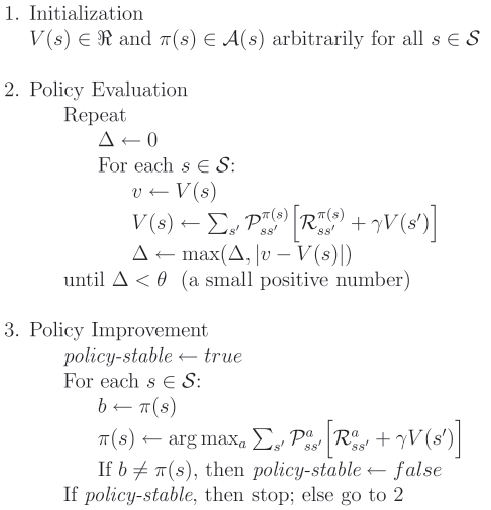
\includegraphics[width=0.5\textwidth]{Bilder/Policy.png}
	\caption{Algorithmus zur Policy Iteration}
	\label{fig:Policy}
\end{figure}


\subsection{Value Iteration}
Betrachtet man die Policy Iteration stellt man fest, dass jeder Schritt die lange Bewertung (Evaluation) der Policy beinhaltet, in der eine iterative Berechnung über alle Zustände geschieht. Die iterativen Evaluation bricht erst ab, wenn es nach $V^{\pi}$ konvergiert, doch so lange muss gar nicht gewartet werden. Die Policy Iteration, kann in vielen Fällen beschränkt werden, ohne die Konvergenz zu verlieren, welche durch die Policy Iteration garantiert wird. Ein Spezialfall ist das \textbf{Stoppen der Evaluation nach einem Durchgang} (alle Zustände wurden einmal gespeichert \glqq backuped\grqq\xspace), welcher als Value Iteration bezeichnet wird.\\
\\
Hierbei wird die Backup-Operation mit dem Improvement der Policy kombiniert und man erhält die Formel:

\begin{equation}
V_{k+1}(s) = max_{a} \sum_{s^{'}} P^a_{ss^{'}} [R^a_{ss^{'}} + \gamma V_{k} (s^{'})]
\end{equation}

Die Value Iteration kombiniert effektiv Evaluation und Improvement, der Algorithmus ist Abbildung \ref{fig:Value} zu entnehmen.

\begin{figure}[htbp]
	\centering	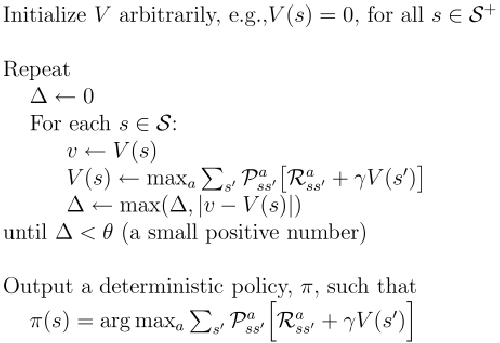
\includegraphics[width=0.5\textwidth]{Bilder/Value.png}
	\caption{Algorithmus zur Value Iteration}
	\label{fig:Value}
\end{figure}

\subsection{Gemeinsamkeiten und Unterschiede von Policy und Value Iteration}
\label{sec:dynamic_programming_unterschiede}
Zuerst soll hier nochmal auf die Gemeinsamkeit von Policy und Value Iteration eingegangen werden. 
Da beides Verfahren der Dynamischen Programmierung sind, benötigen sie ein vollständiges Modell der Welt bzw. der Umgebung.
Es müssen also die direkte Belohnung $r$ und der Nachfolgezustand $s_{t+1}$ (welcher durch eine Funktion $s_{t+1} = \delta(s,a)$ bestimmt wird) zur Durchführung der Policy Evaluation Phase (bzw. Berechnung der State-Value-Function $V^{\pi}$) für beiden Verfahren bekannt sein.

\subsubsection{Konzeptionelle Unterschiede}
Wie bereits erwähnt, entfällt bei der Value Iteration das wiederholte Optimieren der Strategie $\pi$ bis diese konvergiert.
Aber warum kann man dies überhaupt wegfallen lassen?\\

\begin{figure}[htbp]
	\centering	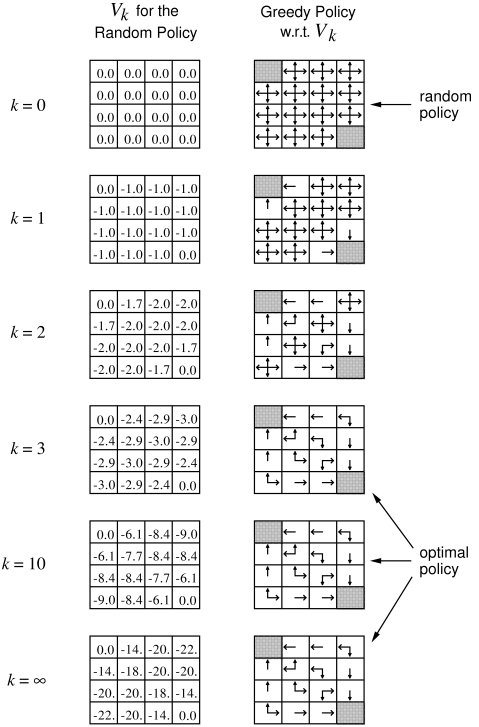
\includegraphics[width=0.5\textwidth]{Bilder/KonvergenzVkPolicy}
	\caption{Zusammenhang zwischen der Konvergenz von $V_{k}$ und der optimierten Policy $\pi^{'}$ }
	\label{fig:konvergenz}
\end{figure}

Hierzu muss man das Konvergenzverhalten der State-Value-Function $V_{k}$ und einer Policy $\pi^{'}$ betrachten.
Dieses ist in der Abbildung \ref{fig:konvergenz} für eine Gridworld und eine Greedy Policy, welche es zu optimieren gilt, dargestellt.
In der Abbildung wurde nach jedem Schritt in der Policy Evaluation die Strategie $\pi(s)$ für jedes $s \in S$ optimiert.\\
Hierbei fällt auf, dass man bereits nach dem dritten Policy Evaluation Schritt eine optimale Strategy $\pi^{*}$ erreicht hat. 
Da der Algorithmus für die Policy Iteration in der Policy Evaluation Phase (vgl. Abbildung \ref{fig:Policy}) bis zur Konvergenz (also sehr oft) die State-Value-Function $V$ berechnet, kann davon ausgegangen werden, dass man bereits nach einer Policy Evaluation Phase die optimale Strategie $\pi^{*}$ gefunden hat.\\
Auf Grund dieser Beobachtung kann die Policy Improvement Phase in der Value Iteration so optimiert werden, dass man für alle $s \in S$ nur noch die optimale Aktion $a$ anhand der Zustands-Werte von $s$ bestimmen muss.
Dies wird im Algorithmus zur Value Iteration (vgl. Abbildung \ref{fig:Value}) mit der Zeile $\pi(s) = argmax_{a} \sum_{s^{'}} P^a_{ss^{'}} [R^a_{ss^{'}} + \gamma V_{k} (s^{'})]$ ausgedrückt.\\

Ein anderer Blickwinkel auf die Value Iteration führt über die Bellman-Optimalitäts-Gleichung $V^{*}(s) = \underset{\text{a}}{max} \sum_{s^{'}} P^a_{ss^{'}} [R^a_{ss^{'}} + \gamma V_{k} (s^{'})]$.
Durch die Auswahl der Aktion mit der größten Belohnung $\underset{\text{a}}{max}$ wird die Konvergenz in der Policy Evaluation Phase deutlich verbessert und es müssen weniger Iterationen (bessere Performance) gemacht werden.\\

Das Ausnutzen der beiden beschriebenen Verbesserungen überführen den Algorithmus der Policy Iteration hin zur Value Iteration. 

\subsection{Anwendung Policy und Value Iteration}
In diesem Abschnitt soll anhand von Beispielen erklärt werden, wie die beiden Algorithmen ihre Berechnung durchführen.

\subsubsection{Beschreibung der Randbedingungen}
\begin{itemize}
	\item Zielzustand: unten rechts
	\item Aktionen: links, rechts, oben, unten
	\item Schrittkosten auf einen Nachbarzustand: -1
	\item Gegen Wand oder Barriere laufen: Position bleib unverändert und Kosten -2
	\item Discountfaktor: 0,8
	\item Umwelt ist deterministisch
	\item Initiale Situation: Zufallsstrategie, alle Werte auf 0
\end{itemize}

Es sind jeweils die nächsten beiden Iterationen der Verfahren zu berechnen.

\subsubsection{Policy Iteration}
\label{sec:anwendung_policy_iteration}

\begin{figure}[htbp]
	\centering	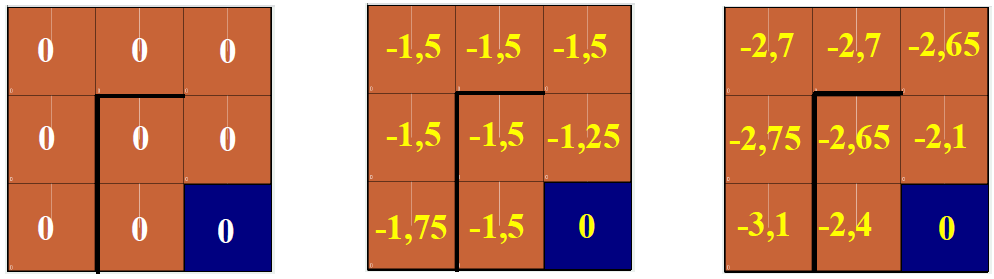
\includegraphics[width=0.5\textwidth]{Bilder/PolicyIterationAufgabe}
	\caption{Ausgangssituation und die beiden folgenden Iterationen bei der Policy Iteration}
	\label{fig:policy_aufgabe}
\end{figure}

Zur Berechnung der Zustands-Werte verwenden wir die folgende Formel aus der Policy Evaluation Phase:
\begin{equation}
V_{k+1}(s) = \sum_{a} \pi(s,a) \sum_{s^{'}} P^a_{ss^{'}} [R^a_{ss^{'}} + \gamma V_{k} (s^{'})]
\end{equation}

Im Folgendem wir die Berechnung der Werte für der ersten Iteration für einige Zustände beispielhaft durchgeführt.
Hierzu werden die Zustände von links-oben nach rechts-unten und von Links nach Rechts durchnummeriert.
Links-oben ist damit Zustand 1 und der Zielzustand ist Zustand Nummer 9.\\

Berechnung Zustand 1:
\begin{align}
	s1^{'} &= \frac{1}{4} * [(-2 + 0,8 * 0) + (-2 + 0,8 * 0) + (-1 + 0,8 * 0) + (-1 + 0,8 * 0)\\
	s1^{'} &= \frac{1}{4} * [ -2 + -2 + -1 + -1 ] = -1,5
\end{align}
Da bei der zugrundeliegenden Zufallsstrategie jede Aktion eine identische Wahrscheinlichkeit besitzt (alle $\frac{1}{4}$) kann die Wahrscheinlichkeit aus der Summe in der eckigen Klammer herausgezogen werden.
Damit entspricht die $\frac{1}{4}$ dem Ausdruck $\sum_{a} \pi(s,a)$. 
Da es sich um eine deterministische Umwelt handelt, ist die Wahrscheinlichkeit für den Übergang von $s$ nach $s^{'}$ ($P^a_{ss^{'}}$) immer 1 und damit in der Berechnung nicht ersichtlich ($\frac{1}{4}$ würde mit 1 multipliziert werden).\\
Die Summe $\sum_{a}$ stellt das Auswerten aller Aktionen $a$ dar.
Jeder Ausdruck in den runden Klammern entspricht einer Aktion, die Reihenfolge in der vorgegangen wurde lautet: links, oben, rechts, unten.\\
Innerhalb der runden Klammer wird für jeder Aktion der direkte Reward $R^a_{ss^{'}}$ und das Produkt aus Discountingfaktor und Wert des nächsten Zustands $\gamma V_{k} (s^{'})$ berechnet.
Im Beispiel wird bei der Aktion "`links"' ein Reward von -2 und und der Wert von $s1$, da wir mit der Aktion außerhalb der Umwelt landen und in $s1$ verbleiben, genommen.
Ansonsten würde der Wert des Zustands $s^{'}$ genommen, dies ist z.B. der Fall für die Aktion "`rechts"' im Zustand $s1$.\\

Für den Zustand 6 gestaltet sich die Berechnung wie folgt:
\begin{align}
	s6^{'} &= \frac{1}{4} * [(-1 + 0,8 * 0) + (-1 + 0,8 * 0) + (-2 + 0,8 * 0) + (-1 + 0,8 * 0)\\
	s6^{'} &= \frac{1}{4} * [ -1 + -1 + -2 + -1 ] = -1,25
\end{align}

Für die zweite Iteration wird der Wert für den Zustand s6 mit den gerade berechneten Zustands-Werten ermittelt (full backup):
\begin{align}
	s6^{''} &= \frac{1}{4} * [(-1 + 0,8 * -1,5) + (-1 + 0,8 * -1,5) + (-2 + 0,8 * -1,25) + (-1 + 0,8 * 0)\\
	s6^{''} &= \frac{1}{4} * [ -2,2 + -2,2 + -3 + -1 ] = -2,1
\end{align}

In der Policy Evaluation Phase würde man anschließen solange iterieren bis die Zustands-Werte konvergieren und dann mit der Policy Improvement Phase beginnen.\\
In ihr wird für alle Zustände $s \in S$ die optimale Aktion über 
$argmax_{a} \sum_{s^{'}} P^a_{ss^{'}} [R^a_{ss^{'}} + \gamma V_{k} (s^{'})]$ bestimmt. 
Danach wird die verbesserte Policy $\pi(s)$ mit der vorherigen Policy $b$ verglichen.
Sollten sich noch Änderungen ergeben haben, wird eine neue Iteration mit Policy Evaluation und Policy Improvement begonnen.
Unterscheiden sich die beiden Policies nicht, so wurde die optimale Strategie gefunden.\\

Abschließend ein Beispiel zur Bestimmung der optimalen Aktion für einen Zustand. Zur Aktionsbestimmung wird die Gleichung $\pi(s) = argmax_{a} \sum_{s^{'}} P^a_{ss^{'}} [R^a_{ss^{'}} + \gamma V_{k} (s^{'})]$ benutzt, welche unter allen Aktionen $a$ im Zustand $s$ diejenige Aktion mit dem größten Wert wählt. Hier am Beispiel des Zustands $s6$ nach Iteration 2 durchgeführt:
\begin{align}
	\pi(s6) &= argmax_{\text{\{links, oben, rechts, unten\}}} \sum_{s^{'}} P^a_{ss^{'}} [R^a_{ss^{'}} + \gamma V_{k} (s^{'})]\\	
	\pi(s6) &= argmax \{ -1 + 0,8 * -2,65; -1 + 0,8 * -2,65; -2 + 0,8 * -2,1; -1 + 0,8 * 0 \}\\
	\pi(s6) &= argmax \{ -3,12; -3,12; -3,68; -1 \}\\
	\pi(s6) &= unten
\end{align}

Am Ergebnis erkennt man dass für den Zustand $s6$ bereits nach der zweiten Iteration die optimale Policy gefunden wurde.
Diesen Schritt würde man in der Policy Improvement Phase für alle Zustände $s$ durchführen und dann überprüfen ob sich Änderungen gegenüber der vorherigen Policy ergeben haben.

\subsubsection{Value Iteration}
\label{sec:anwendung_value_iteration}

Wie bereits im Abschnitt \ref{sec:dynamic_programming_unterschiede} erwähnt wurde, wird bei der Value Iteration in jedem Zustand die Aktion mit der größten Belohnung $V^{*}(s) = \underset{\text{a}}{max} \sum_{s^{'}} P^a_{ss^{'}} [R^a_{ss^{'}} + \gamma V_{k} (s^{'})]$ bestimmt und so eine schnellere Konvergenz im Vergleich zur Policy Iteration erreicht.\\
In diesem Abschnitt wird dieses Verfahren, analog zu der in Abschnitt \ref{sec:anwendung_policy_iteration} beschriebenen Aufgabenstellung, beispielhaft für zwei aufeinander folgenden Iterationen erläutert.
Die Ausgangssituation und die Ergebnisse sind in Abbildung \ref{fig:value_aufgabe} dargestellt.
Zum Vergleich wird hier auch der selbe Zustand $s6$ wie bei der Value Iteration betrachtet.\\ 

\begin{figure}[htbp]
	\centering	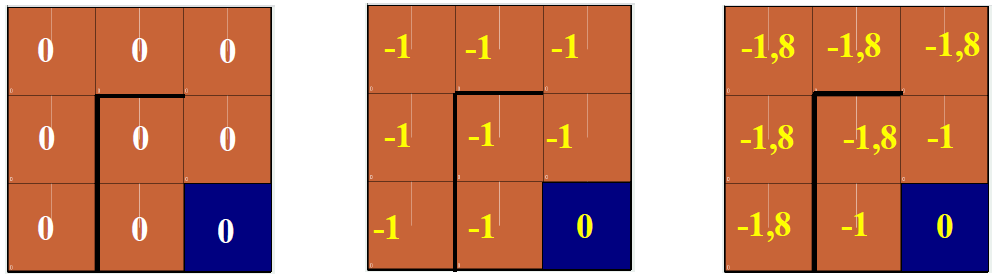
\includegraphics[width=0.5\textwidth]{Bilder/ValueIterationAufgabe}
	\caption{Ausgangssituation und die beiden folgenden Iterationen bei der Value Iteration}
	\label{fig:value_aufgabe}
\end{figure}

Zur Berechnung der Aktion mit der größten Belohnung gehen wir von der Formel $\underset{\text{a}}{max} \sum_{s^{'}} P^a_{ss^{'}} [R^a_{ss^{'}} + \gamma V_{k} (s^{'})]$ aus.
Man betrachtet dabei in jeder Iteration alle Zustände und pro Zustand werden die direkten Belohnungen für alle Aktionen und die Zustandsbewertungen aus der vorherigen Iteration $V_{k}(s^{'})$ betrachtet.
Für die erste Iteration und Zustand $s6$ sieht das wie folgt aus:

\begin{align}
	\underset{\text{a}}{max} = \begin{cases} 
		-1 + 0,8 * 0 & \text{links} \\ 
		-1 + 0,8 * 0 & \text{oben} \\
		-2 + 0,8 * 0 & \text{rechts} \\
		-1 + 0,8 * 0 & \text{unten} \\ 
 	\end{cases}\\
 	\underset{\text{a}}{max} = \begin{cases} 
		-1 & \text{links} \\ 
		-1 & \text{oben} \\
		-2 & \text{rechts} \\
		-1 & \text{unten} \\ 
 	\end{cases}\\
 	\underset{\text{a}}{max} = \{ link, oben, unten \} = -1
\end{align}

Im Zustand $s6$ liefern die Aktionen $ links, oben, unten$ die größte direkte Belohnung von $-1$ so dass $V_{k+1}(s) = -1$ ist.
Für die zweite Iteration wird genau so vorgegangen:
\begin{align}
	\underset{\text{a}}{max} = \begin{cases} 
		-1 + 0,8 * -1 & \text{links} \\ 
		-1 + 0,8 * -1 & \text{oben} \\
		-2 + 0,8 * -1 & \text{rechts} \\
		-1 + 0,8 * 0 &  \text{unten} \\ 
 	\end{cases}\\
 	\underset{\text{a}}{max} = \begin{cases} 
		-1,8 & \text{links} \\ 
		-1,8 & \text{oben} \\
		-2,8 & \text{rechts} \\
		-1 & \text{unten} \\ 
 	\end{cases}\\
 	\underset{\text{a}}{max} = \{ unten \} = -1
\end{align}

In diesem Fall ändert sich an dem für $V_{k+1}(s)$ berechneten Wert nichts, jedoch ist jetzt klar dass im Zustand $s6$ die Aktion $unten$ die optimale Aktion mit der größten Belohnung ist.
Dieses könnte auch nochmal mit der Formel $\pi(s6) = argmax_{\text{\{links, oben, rechts, unten\}}} \sum_{s^{'}} P^a_{ss^{'}}$ nach der Konvergenz der Zustands-Werte explizit berechnet werden.\\
Hier zum Vergleich, dass sich bei der Berechnung die Zustands-Werte auch ändern können, die beiden Iteration für den Zustand $s5$:
\begin{align}
	\underset{\text{a}}{max} = \begin{cases} 
		-2 + 0,8 * 0 & \text{links} \\ 
		-2 + 0,8 * 0 & \text{oben} \\
		-1 + 0,8 * 0 & \text{rechts} \\
		-1 + 0,8 * 0 & \text{unten} \\ 
 	\end{cases}\\
 	\underset{\text{a}}{max} = \begin{cases} 
		-2 & \text{links} \\ 
		-2 & \text{oben} \\
		-1 & \text{rechts} \\
		-1 & \text{unten} \\ 
 	\end{cases}\\
 	\underset{\text{a}}{max} = \{ rechts, unten \} = -1
\end{align}

\begin{align}
	\underset{\text{a}}{max} = \begin{cases} 
		-2 + 0,8 * -1 & \text{links} \\ 
		-2 + 0,8 * -1 & \text{oben} \\
		-1 + 0,8 * -1 & \text{rechts} \\
		-1 + 0,8 * -1 & \text{unten} \\ 
 	\end{cases}\\
 	\underset{\text{a}}{max} = \begin{cases} 
		-2,8 & \text{links} \\ 
		-2,8 & \text{oben} \\
		-1,8 & \text{rechts} \\
		-1,8 & \text{unten} \\ 
 	\end{cases}\\
 	\underset{\text{a}}{max} = \{ rechts, unten \} = -1,8
\end{align}

Auch in für diesen Zustand hat man nach der zweiten Iteration bereits die optimale Strategie gefunden. 
Im Zustand $s5$ ist es nämlich egal ob man $rechts$ oder nach $unten$ geht,so dass damit die optimalen Aktionen ${rechts, unten}$ sind.

\section{Monte Carlo Methoden}
\label{sec:monteCarloMethoden}

\subsection{Grundidee}
Bei den Monte Carlo Methoden besitzt man kein vollständiges Wissen über die Umgebung, sondern sammelt Erfahrungen durch tatsächliches oder simuliertes Interagieren mit der Umwelt. Zudem gibt es nur episodische Aufgaben, da die Belohnung sichergestellt sein muss. Die Abschätzung der Zustandswerte und Strategie-Änderungen geschieht erst am Ende einer Episode (Wert eines Zustandes = kumulierte Belohnung bis zum Ende der Episode). Am Ende wird der Durchschnitt über alle Episoden gebildet.\\
\\
Vorteile gegenüber Dynamic Programming:
\begin{itemize}
\item{Das optimale Verhalten kann direkt aus der Interaktion mit der Umgebung gelernt werden, ohne ein Modell der Umgebung vorhalten zu müssen.}
\item{Sie können in Simulationen oder Beispiel-Modellen eingesetzt werden, man muss also kein komplettes Umgebungsmodell mit den Übergangswahrscheinlichkeiten erstellen.}
\item{Es ist einfach und effizient sich mittels der Monte Carlo Methoden auf eine kleine Teilmenge der Zustände zu fokussieren.}
\end{itemize}

Trotz der Unterschiede zwischen Dynamic Programming und Monte Carlo Methoden, werden die wichtigsten Ideen vom Dynamic Programming übernommen. Es werden die gleichen Value-Functions berechnet und über die gleichen Methoden versucht, die optimale Funktion zu bestimmen. Beim Dynamic Programming werden in der Evaluation $V^{\pi}$ und $Q^{\pi}$ für eine Policy $\pi$ bestimmt und anschließen durch Improvement verbessert. Jeder dieser Schritte wird für die Monte Carlo Methoden übernommen, in dem nur beispielhafte Erfahrungen vorhanden sind, da die Umgebung unbekannt ist.

\subsection{Abgrenzung: Monte-Carlo-Simulation}
Verfahren aus der Stochastik in dem sehr häufig durchgeführte Zufallsexperimente die Basis darstellen. Ziel ist es analytisch nicht oder zu sehr aufwändig lösbare Probleme mit Hilfe der Wahrscheinlichkeitstheorie numerisch zu lösen. Die Grundlage bildet das Gesetz der Großen Zahlen, wobei computergenerierte Vorgänge den Prozess in ausreichend häufigen Zufallsereignissen simulieren können.

\subsection{Policy Evaluation}
\subsubsection{Schätzung der State-Values $V^{\pi}(s)$}
Wie in den Abschnitten zuvor bereits erwähnt, ist der Wert eines Zustandes, der erwartete zukünftige kumulierte discounted reward, ausgehend vom betrachteten Zustand. Eine Möglichkeit diesen Wert aus Erfahrungen zu schätzen, ist es die erhaltenen Belohnungen zu mitteln, nachdem der Zustand besucht wurde. Je mehr Belohnungen für diesen Zustand beobachtet werden, desto näher sollte das Mittel zum erwarteten Wert konvergieren. Diese Idee verfolgen alle Monte Carlo Methoden.\\
Beide Verfahren First- und Every-visit MC konvergieren nach $V^{\pi}(s)$, wenn die Anzahl der Besuche ins unendliche geht (Gesetz der großen Zahlen).

\subsubsection{Every-visit Monte Carlo}
Die Every-visit MC Methode schätzt man $V^{\pi}(s)$ über die Mittelwertbildung aller Belohnungen, die bei \textbf{jedem Besuch} vom Zustand $s$ in einer Episode erhalten werden.

\subsubsection{First-visit Monte Carlo}
Innerhalb einer Episode wird der \textbf{erste Besuch} von $s$ als First-visit bezeichnet und die First-visit MC Methode bildet den Mittelwert nur über die ersten Besuche von $s$ innerhalb einer Episode.\\
Der Algorithmus wird in Abbildung \ref{fig:FirstVisit} dargestellt. Es wird eine Episode für die Strategie $\pi$ ausgeführt und für jeden Zustand $s$ der Episode wird die Belohnung $R$ festgehalten, die dem ersten Besuch von $s$ folgt. $R$ wird anschließend zu den aus vorherigen Episoden erhaltenen Rewards $Returns(s)$ addiert, woraufhin die Rewards gemittelt und $V^{\pi}(s)$ zugewiesen werden.

\begin{figure}[htbp]
	\centering	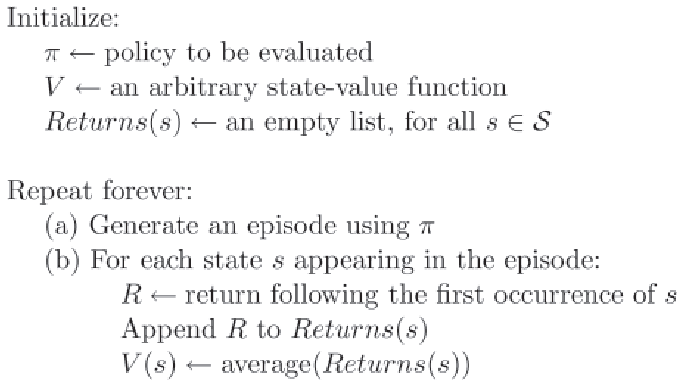
\includegraphics[width=0.8\textwidth]{Bilder/First-visit_MC.png}
	\caption{First-visit MC Algorithmus zur Bestimmung von $V^{\pi}(s)$}
	\label{fig:FirstVisit}
\end{figure}

\subsubsection{Schätzung der Action-Values $Q^{\pi}(s,a)$}
Beim Dynamic Programming haben wir ein komplettes Modell der Umwelt und können hinreichend anhand der State-values entscheiden, welche Policy die geeignetste ist, indem wir immer einen Schritt voraus schauen und die Aktion wählen, die uns zu der besten Kombination aus Reward und Folgezustand bringt.\\
Ohne dieses Modell benötigen wir zwingend die Schätzung der Aktionen um eine Policy bewerten zu können, deswegen ist eines der Hauptziele $Q^{*}$ zu schätzen.\\
\\
Das Problem hierbei ist alle möglichen $Q^{\pi}(s,a)$ zu schätzen. Die Methoden um einzelne $Q^{\pi}(s,a)$ Werte zu schätzen erfolgt genauso wie in den oben genannten First- und Every-visit Verfahren, wobei entweder das erste Auftreten des Zustandes $s$ mit Auswahl der Aktion $a$ oder jedes Auftreten der Kombination $s$ und $a$ über alle Episoden gemittelt wird. Auch hier konvergieren die Werte mit größer werdender Anzahl der Episoden.\\
Das Problem hierbei ist, dass möglicherweise nicht alle Kombinationen aus Zustand $s$ und Aktion $a$ besucht werden. \textbf{Wenn $\pi$ eine deterministische Strategie ist, dann wird man nur jeweils eine Aktion pro Zustand beobachten} und die Erfahrung für andere Aktionen in dem entsprechenden Zustand wird sich nicht verbessern, da diese nicht betrachtet werden.\\
Dies ist ein großes Problem, da es der Zweck der Action-value-function $Q^{\pi}(s,a)$ ist, in einem Zustand die richtige Aktion auswählen zu können. Um die verschiedenen Aktionen jedoch vergleichen zu können, müssen mit \textbf{allen Aktionen Erfahrungen gesammelt} worden sein.\\
\\
Dieses \textbf{\glqq maintaining exploration\grqq\xspace Problem}, dass für die Nutzung der Action-values die kontinuierliche Exploration sichergestellt sein muss, kann dadurch gelöst werden, dass jeder erste Schritt der Episode an einem zufälligen State-Action-Pair startet und jedes State-Action-Pair eine Wahrscheinlichkeit $\geq 0$ hat ausgewählt zu werden. Diese Annahme wird \textbf{Exploring starts} genannt.

\subsection{Policy Improvement}
\subsubsection{Generalized Policy Iteration}
Die Idee hinter der Generalized Policy Iteration (GPI) ist die gleiche wie beim Dynamic Programming, nur dass hier anstelle der State-Value-Function $V$ die Action-Value-funtion $Q$ verwendet wird.\\
Man hält jeweils eine approximierte Policy $\pi$ und Action-Value-funtion $Q$ vor. Die Action-Value-funtion wird immer wieder angepasst, sodass sie die Value-function der Policy besser approximiert und die Policy wird immer wieder auf Basis der Action-Value-funtion verbessert (vgl. Abbildung \ref{fig:MC_GPI}).

\begin{figure}[htbp]
	\centering	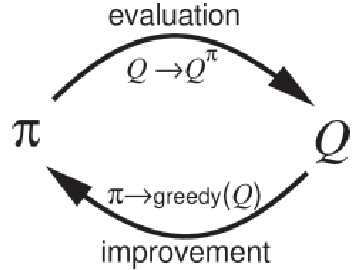
\includegraphics[width=0.5\textwidth]{Bilder/MC_GPI.png}
	\caption{Generalized Policy Iteration}
	\label{fig:MC_GPI}
\end{figure}

\subsubsection{Monte Carlo ES (Exploring Starts)}
Für die Monte Carlo Methoden ist es natürlich, dass die Bewertung (evaluation) und Verbesserung (improvement) zwischen den Episoden stattfindet. Nach jeder Episode werden die beobachteten Returns genutzt um die Strategie zu bewerten und danach wird die Strategie für alle besuchten Zustände in der Episode verbessert. Der Algorithmus hierzu wird in Abbildung \ref{fig:MC_ES} gezeigt.

\begin{figure}[htbp]
	\centering	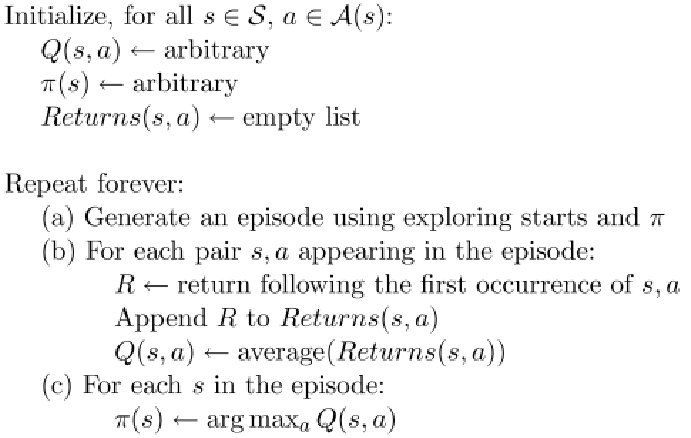
\includegraphics[width=0.8\textwidth]{Bilder/MC_ES.png}
	\caption{Monte Carlo Exploring Starts Algorithmus}
	\label{fig:MC_ES}
\end{figure}

Der Algorithmus startet damit, dass $Q(s,a)$ und die Policy $\pi$ zufällig gewählt werden (exploring starts), sodass alle möglichen Kombinationen von $s$ und $a$ untersucht werden. Ähnlich wie beim First-visit MC in Abbildung \ref{fig:FirstVisit}, wird der Return des ersten Auftretens von Zustand $s$ und Aktion $a$ gespeichert und zu den bereits über alle Episoden beobachteten Belohnungen $Returns(s,a)$ addiert. Es folgt die Bildung des Mittelwertes für $Q(s,a)$ unabhängig davon welche Policy zum Zeitpunkt der Beobachtung aktiv war. Damit ist die Evaluation (b) beendet und es beginnt das Improvement (c) bei dem für einen Zustand $s$ die Aktion in der Policy $\pi$ hinterlegt wird, die den größten Wert $Q(s,a)$ hat.\\


\subsubsection{On-Policy Monte Carlo}
Beim zuvor vorgestellten Ansatz \glqq MC mit Exploring Starts\grqq\xspace wurde mittels zufälliger Wahl verschiedener Anfangszustände $s$ und Aktionen $a$ versucht, alle möglichen Kombinationen abzudecken. Dies ist aber eine unrealistische Annahme die so in der Realität nicht erfüllt werden kann. Der einzige Weg um sicherzustellen, dass alle Aktion unendlich häufig getestet werden ist der, dass der Agent diese auch weiterhin nutzt (nicht nur beim Start).\\
Es gibt zwei Ansätze die dies sicherstellen, die On-Policy und Off-Policy Verfahren, von denen hier zunächst das erste vorgestellt wird.\\
\\
On-Policy Verfahren versuchen die Strategie zu bewerten und zu verbessern die genutzt wird um Entscheidungen zu treffen.\\
Bei den den On-Policy Methoden gibt es \textbf{nur eine Strategie}, die über den nächsten Schritt entscheidet. Diese \textbf{Policy ist generell soft} was bedeutet, dass $\pi(s,a) > 0$ für alle $s \in S$ und $a \in A(s)$ (alle Kombinationen aus Zustand und Aktion sind vorhanden). In dem hier vorgestellten Algorithmus unter Abbildung \ref{fig:MC_OnPolicy} kommt eine \textbf{$\epsilon$-greedy Policy} zu Einsatz, die die meiste Zeit diejenige Aktion auswählt, die den größten erwarteten Gewinn verspricht und mit einer Wahrscheinlichkeit $\epsilon$ eine zufällige Aktion auswählt. Dadurch erhält man einen \textbf{Nichtdeterminismus bei der Auswahl von Aktionen}, wodurch alle Aktionen $a$ für einen Zustand $s$ gewählt werden können. $\epsilon$-greedy Strategien sind dabei ein Spezialfall von \textbf{$\epsilon$-soft Strategien} für die gilt $\pi(s,a) \geq \frac{\epsilon}{|A(s)|}$ für alle $s \in S$ und $a \in A(s)$ mit $\epsilon > 0$ (hierbei steht $\frac{\epsilon}{|A(s)|}$ für die Wahrscheinlichkeit aller Aktionen außer der günstigsten im Zustand $s$). Die günstigste Aktion erhält die Restwahrscheinlichkeit $1-\epsilon + \frac{\epsilon}{|A(s)|}$.\\
\\
Die Grundidee vom On-Policy Monte Carlo ist die gleiche wie bei der Generalized Policy Iteration (GPI). Es wird die First-visit MC Methode genutzt um die Action-value-function die Policy zu bestimmen, jedoch kann man nicht einfach die Policy auf Grundlage der Action-value-function verbessern, da dies dazu führen würde, dass nicht mehr alle Zustände exploriert würden. \textbf{Deswegen wird die Policy anstatt sie zu einer greedy Policy zu machen nur zu einer $\epsilon$-greedy Policy gemacht.} Für jede $\epsilon$-soft Policy $\pi$ ist garaniert, dass jede $\epsilon$-greedy Policy auf Basis von $Q^{\pi}$ besser oder gleich $\pi$ ist (sichergestellt durch das Policy Improvement Theorem).

\begin{figure}[htbp]
	\centering	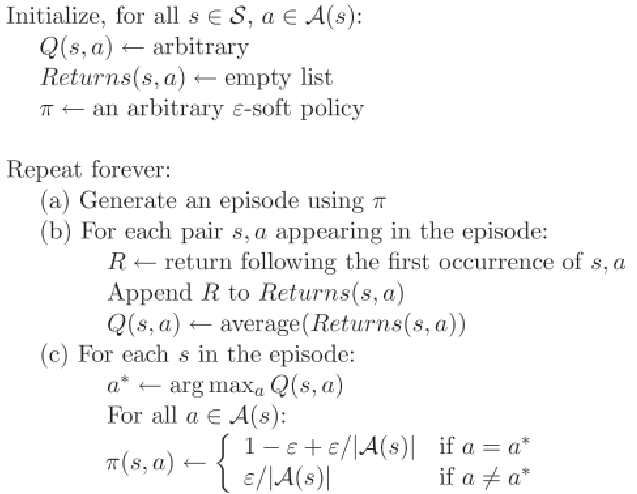
\includegraphics[width=0.8\textwidth]{Bilder/MC_OnPolicy.png}
	\caption{$\epsilon$-soft On-Policy Monte Carlo Algorithmus}
	\label{fig:MC_OnPolicy}
\end{figure}

\subsubsection{Off-Policy Monte Carlo}
Es sein angenommen, dass $V^{\pi}$ und $Q^{\pi}$ geschätzt werden sollen, aber nur Episoden der Policy $\pi'$ vorhanden sind, wobei gilt $\pi' \neq \pi$. Das Lernen einer Value-function für eine Policy $\pi$ auf Basis der Erfahrungen, die durch eine andere Policy $\pi'$ gesammelt wurden nennt man Off-Policy Verfahren.\\
\\
Im Verglich zum On-Policy Verfahren mit dem charakteristischen Feature, dass der Wert einer Policy dadurch geschätzt wird, indem man sie zur Kontrolle verwendet, werden beim Off-Policy Verfahren diese beiden Funktionen getrennt.\\
Die Strategie die genutzt wird um Verhalten zu generieren wird \textbf{behaviour policy} genannt und ist evt. gar nicht abhängig von der Strategie welche bewertet (evaluated) und verbessert (improved) wird  \textbf{estimation policy}. Vorteil dieser Trennung ist, dass die \textbf{estimation Policy deterministisch} sein kann, währen die\textbf{ behaviour policy weiterhin alle möglichen Aktionen ausprobieren} kann.\\
Der Algorithmus folgt dabei der behaviour policy und verbessert die estimation Policy. Um alle Möglichkeiten zu untersuchen muss, die \textbf{behaviour policy soft} sein. Abbildung \ref{fig:MC_OffPolicy} zeigt einen Off-Policy Monte Carlo Algorithmus.

\begin{figure}[htbp]
	\centering	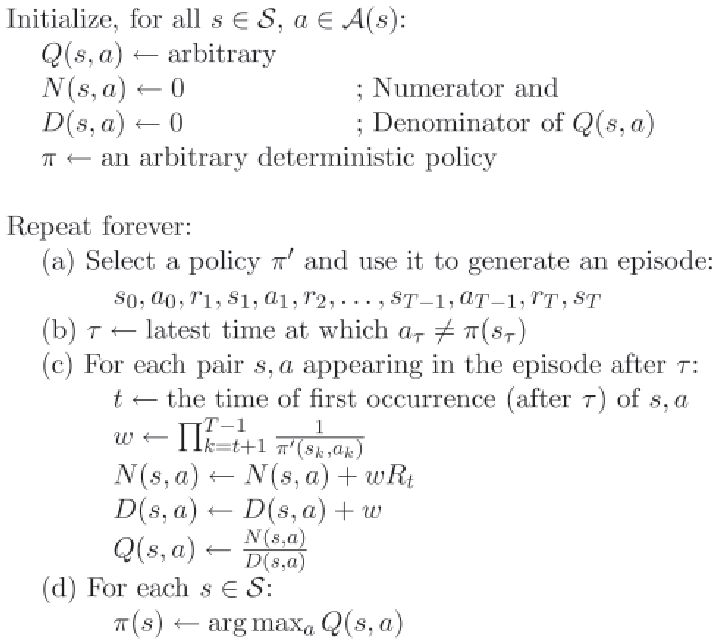
\includegraphics[width=0.8\textwidth]{Bilder/MC_OffPolicy.png}
	\caption{Off-Policy Monte Carlo Algorithmus}
	\label{fig:MC_OffPolicy}
\end{figure}

Die behaviour policy $\pi'$ ist eine willkürliche soft policy. Die estimation policy $\pi$ ist greedy auf Basis von $Q$ und eine Schätzung von $Q^{\pi}$.

\section{Temporal-Difference Learning}
	\subsection{Motivation}
	Dynamic Programming (siehe: \ref{sec:dynamicPrograming}) und Monte Carlo Methoden (siehe: \ref{sec:monteCarloMethoden}) weisen Einschränkungen auf die im praktischen Einsatz die Größe der lösbaren Probleme stark einschränken. Dies sind im einzelnen:
	\begin{description}
		\item[DP]{Die Menge der Zustände ist bekannt und endlich}
		\item[DP]{Die Menge der möglichen Aktionen \{a\} ist bekannt und endlich}
		\item[DP]{Die Belohnungen für alle Zustände müßen bekannt sein}
		\item[DP]{Die Folgezustände in Abhängigkeit von Ausgangszustand und Aktion müßen bekannt sein}
 		\item[DP]{Die Menge der Zustände muß bekannt und endlich sein}
		\item[MC]{Das Problem muß episodisch sein}
		\item[MC]{Wissen aus vorhergehenden Episoden wird nicht verwendet (Rechenaufwand)}
	\end{description}
	
	Temporal Difference Learning verbindet Konzepte der Dynamischen Programmierung und der Monte Carlo Methoden um die Nachteile zu vermeiden und die Vorteile (s.u.) der jeweiligen Methode beizubehalten.
	
	\begin{description}
		\item[MC] Zustandraum kann zur Laufzeit erforscht werden
		\item[DP] Verteilung der Belohnungen auf die korrekten, die ``verantwortlichen`` Zustände
	\end{description}


	\subsection{Arbeitsweise Umgangssprachlich}
	Der Gedank bei Temporal Difference Learning alle Erwartungswerte für rewards beliebig zu füllen und dann beim durchlaufen eine Pfades die auf diesem liegenden Werte anhand ihrer der Abweichung $real - erwartet$ anzugleichen.

\subsection{On-Policy TD Control: Sarsa}

Im ersten Schritt wird die \glqq action-value-function\grqq\xspace $Q^{\pi}(s,a)$ für die aktuelle Strategie $\pi$ und alle Zustände $s$ und Aktionen $a$ gelernt. Man erhält somit eine alternierende Sequenz aus Zuständen und Zustands-Aktions Paaren (state-action-pairs), die in Abbildung \ref{fig:SA-Pairs} dargestellt ist.

\begin{figure}[htbp]
	\centering	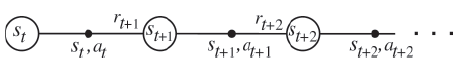
\includegraphics[width=0.8\textwidth]{Bilder/OnPolicy.png}
	\caption{Sequenz aus states und state-action-pairs}
	\label{fig:SA-Pairs}
\end{figure}

Aus diesen Übergängen von state-action-pair zu state-action-pair werden die Belohnungen ermittelt, um den Wert der state-action-pairs zu bestimmen.

\begin{equation}
Q(s_{t},a_{t}) \leftarrow Q(s_{t},a_{t}) + \alpha [r_{t+1} + \gamma Q(s_{t+1},a_{t+1}) - Q(s_{t},a_{t})]
\end{equation}

Der Wert $\alpha$ ist hierbei ein konstanter Parameter für die Schrittweite. Der Sarsa-Algorithmus ist ein On-Policy Control Algortihmus und wird in Abbildung \ref{fig:Sarsa} dargestellt.

\begin{figure}[htbp]
	\centering	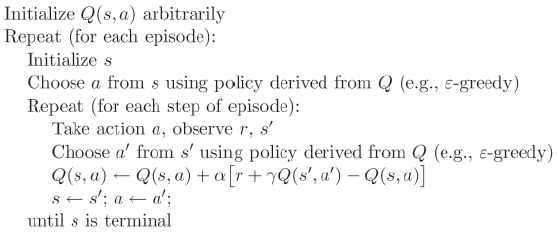
\includegraphics[width=0.8\textwidth]{Bilder/Sarsa.png}
	\caption{Sarsa: On Policy TD Control Algorithmus}
	\label{fig:Sarsa}
\end{figure}


\subsection{Off-Policy TD Control: Q-Learning}
Beim Off-Policy Verfahren approximiert die gelernte \glqq action-value-function\grqq\xspace $Q$  direkt dir optimale Funktion $Q^{*}$ unabhängig davon welche Strategie verfolgt wird. Q-Learning ist ein Off-Policy TD Control Algorithmus und wird in Abbildung \ref{fig:QLearning} dargestellt.
 
\begin{equation}
Q(s_{t},a_{t}) \leftarrow Q(s_{t},a_{t}) + \alpha [r_{t+1} + \gamma max_{a} Q(s_{t+1},a) - Q(s_{t},a_{t})]
\end{equation} 
 
\begin{figure}[htbp]
	\centering	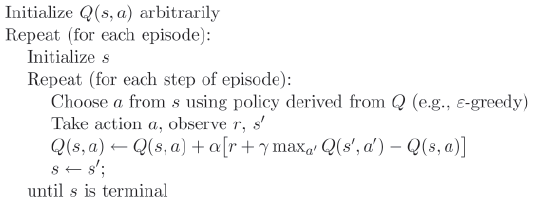
\includegraphics[width=0.8\textwidth]{Bilder/Q-Learning.png}
	\caption{Q Learning: Off Policy TD Control Algorithmus}
	\label{fig:QLearning}
\end{figure}

\subsection{Cliff-Anwendung}
Die Cliff-Anwendung zeigt die Unterschiede zwischen Sarsa (On-Policy) und Q-Learning (Off-Policy) Methoden.\\
Der Agent soll vom Start zum Ziel gelangen und dabei der Klippe nicht zu nahe kommen. Der Agent kann sich nach oben, unten, links und rechts bewegen und wird mit einem Reward von -1 für alle Übergänge belohnt. Wenn er der Klippe jedoch zu nahe kommt, erhält er eine Belohnung von -100 und wird unmittelbar auf den Startpunkt zurück gesetzt (vgl. Abbildung \ref{fig:Cliff}).

\begin{figure}[htbp]
	\centering	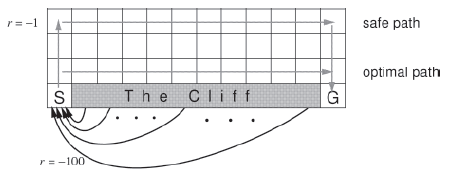
\includegraphics[width=0.8\textwidth]{Bilder/Cliff.png}
	\caption{Cliff Anwendung}
	\label{fig:Cliff}
\end{figure}
\todo{check: Auf der cliff Abbildung \ref{fig:Cliff} sieht der optimale weg aus wie ca. -14 in Abbildung \ref{fig:Cliff_Result} kommt keiner näher als ca. -25 ?}

Die Ergebnisse sind Abbildung \ref{fig:Cliff_Result} zu entnehmen. Q Learning lernt die Werte für die optimale Strategie, wodurch der Agent nahe der Klippe entlangläuft und häufiger herunterfällt. Sarsa hingegen berücksichtigt die Auswahl der Aktionen und lernt den längeren aber sichereren Pfad. Auch wenn Q Learning die optimale Strategie lernt, ist die Performance schlechter als die von Sarsa.\\

\begin{figure}[htbp]
	\centering	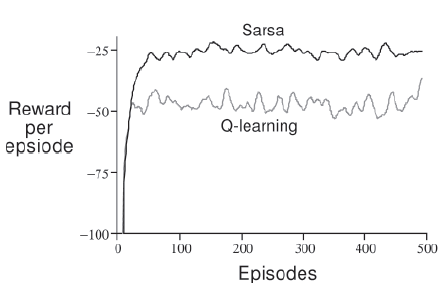
\includegraphics[width=0.8\textwidth]{Bilder/Cliff_Ergebnisse.png}
	\caption{Vergleich Sarsa und Q-Learning}
	\label{fig:Cliff_Result}
\end{figure}

\todo{check: Oben steht das Q Learning den optimalen Pfad lernt, Q Learning hat in Abbildung \ref{fig:Cliff_Result} aber anscheinend einen schlechteren Reward als Sarsa das den sicherreren Pfad lernen soll ?}

\subsection{Trace Decay Factor}
\subsubsection{Zusammenfassung Umgangssprachlich}
Der Trace decay faktor gibt an mit welcher Stärke eine in Zustand $s_t$ beobachtete Abweichung der real gemessen Rewards von den erwarteten Rewards $V(s_t)$ in die erwarteten Rewards der Zustände über die zu $s$ gelangt wurde eingerechnet wird.
Hierzu wird ein Trace Decay Factor $\lambda$ für jeden Zustand geführt der steigt wenn ein Zustand besucht wird und sonst für diesen abnimmt und in der Regel einen Multiplikator $\leq 1$ darstellt. Mit $\lambda$ multipliziert reduziert sich also der in $s_t$ gefunden Fehler für die Zustände $s_{t-n}$ (solche über die zu $s_t$ gelangt wurde) in der Regel wird der Fehler umso mehr abgeschwächt umsoweiter $s_{t-n}$ in der Vergangenheit liegt..

\subsubsection{Referenzen/Bilder}
Der Trace Decay Factor $\lambda$ ist ein \glqq accumulating eligibility trace\grqq\xspace welcher angibt wie häufig ein Zustand besichtigt wurde (vgl. Abbildung \ref{fig:Trace}). Wird ein Zustand weniger häufig besucht nimmt der Faktor über die Zeit hinweg ab.\\
\subsection{Eligibility Traces}
Werden in TD Learning Algorithmen verwendet und ist ein Konzept, um den in einem TD
Schritt errechneten Fehler auch an vorhergehende Schritte weiterzureichen (vgl. Studienarbeit
Markelic Kap 3.4.1).

\begin{figure}[htbp]
	\centering	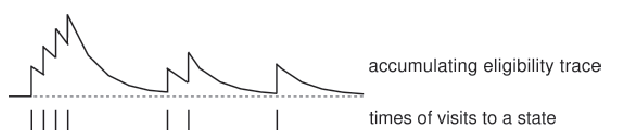
\includegraphics[width=0.8\textwidth]{Bilder/TraceDecay.png}
	\caption{Trace Decay Factor}
	\label{fig:Trace}
\end{figure}

\subsection{Vergleich der Verfahren}
Drei drei vorher vorgestellten Verfahren dynamische Programmierung, Monte-Carlo-Methoden und Temporal Difference Learning werden in diesem Abschnitt nochmal im Hinblick auf ihre Vor- und Nachteile verglichen.

\subsubsection{Dynamic Programming}
Dynamische Programmierung berechnet optimale Strategien auf Basis eines vollständigen Modells der Umgebung. Die Zustände und Zustandsübergänge der Umgebung müssen dabei einen Markov-Entscheidungsprozess darstellen.

\textbf{Voraussetzungen}
\begin{itemize}
\item{Die Menge der Umweltzustände ist bekannt und ist endlich}
\item{Die Menge der möglichen Aktionen \{a\} ist bekannt und endlich}
\item{Belohnungen für alle Umweltzustände bekannt}
\item{Folgezustände in Abhängigkeit von Ausgangszustand und Aktion bekannt}
\end{itemize}

\vspace{1em}
\textbf{Vor- und Nachteile}
\begin{description}
\item[$+$] Findet garantiert eine optimale Strategie in polynomialer Zeit
\item[$+$] Funktioniert bei heutigen Computern mit Millionen von Zuständen
\item[$-$] Es wird ein vollständiges Modell der Umweltzustände, Aktionen und Belohnungen benötigt
\item[$-$] Hoher Rechenaufwand
\item[$-$] Nur für diskrete Zustandsräume verwendbar
\item[$-$] Sehr empfindlich gegenüber Verletzungen der Markov-Eigenschaft, da neue Schätzungen auf vorherigen Schätzungen basieren (\emph{Bootstrapping})
\end{description}

\subsubsection{Monte-Carlo-Methoden}
Monte Carlo Methoden betrachten jeweils nur eine Sequenz von Zustandsübergängen (eine \emph{Experience}) und benötigt daher kein Modell. \todo{Check: Kein Modell oder ein kleineres ? Wir erstellen doch beim TD eigentlich auch ein Modell, wie ist hier die Abgrenzung ? OS}\\

\textbf{Voraussetzungen}
\begin{itemize}
\item Die zu lösende Aufgabe ist episodisch
\end{itemize}

\vspace{1em}
\textbf{Vor- und Nachteile}
\begin{description}
\item[$+$] Kein Modell der Umgebung erforderlich. Stattdessen werden nur Episoden (Sequenzen aus Zuständen, Aktionen und Belohnungen) benötigt, die durch Interaktion mit der Umgebung generiert werden. Diese Episoden können durch einfache Modelle generiert werden, die häufig wesentlich einfacher zu finden sind, als vollständige Modelle der Umwelt mit expliziten Transitionswahrscheinlichkeiten
\item[$+$] Robuster als DP gegenüber Verletzungen der Markov-Eigenschaft. Dies liegt daran, dass neue Schätzungen nicht auf vorherigen Schätzungen basieren (kein \emph{Bootstrapping})
\item[$+$] Monte-Carlo-Methoden fokussieren sehr gut auf eine kleine Teilmenge der Umweltzustände
\item[$+$] Garantierte (asymptotische) Konvergenz zur optimalen Strategie
\item[$-$] Nur für episodische Tasks geeignet, da die Belohnung immer erst am Ende einer Episode generiert wird
\item[$-$] Ausreichende Exploration ist bei deterministischen Strategien ein Problem, da keine alternativen Aktionen getestet werden. Dies kann z.B. durch den Start mit zufälligen Zustands-Aktions-Paaren (sog. \emph{Exploring Starts}) verhindert werden
\end{description}

\subsubsection{Temporal Difference Learning}
Temporal Difference Learning vereint Ideen der dynamischen Programmierung und der Monte-Carlo-Methoden. Es verwendet \emph{Bootstrapping} wie Monte-Carlo-Methoden, benötigt jedoch kein Modell der Umwelt wie die dynamische Programmierung.

\textbf{Voraussetzungen} \\
Keine? \todo{Ich sehe hier keine Vorraussetzungen - jemand von euch? SM}

\vspace{1em}
\textbf{Vor- und Nachteile}
\begin{description}
\item[$+$] Lernen direkt durch Erfahrung, kein Modell der Umwelt mit Zuständen, Zustandsübergängen und Belohnungen notwendig
\item[$+$] Inkrementell wie dynamische Programmierung: Belohnungen nach jedem Schritt, nicht wie bei Monte-Carlo-Methoden erst nach einer Episode. Dadurch meist schneller, vor allem bei langen Episoden
\item[$+$] Auch für nicht-episodische Aufgaben geeignet
\item[$+$] Garantierte (asymptotische) Konvergenz zur optimalen Strategie. Konvergiert erfahrungsgemäß häufig schneller als Monte-Carlo-Methoden (einen formalen Beweis dafür gibt es allerdings nicht)
\item[$+$] Einfachheit: Wenig Rechenaufwand, es werden nur einzelne Gleichungen benötigt, dadurch kleine Programme
\item[$-$] Empfindlich gegenüber Verletzungen der Markov-Eigenschaft, da aktuelle Schätzungen auf vorherigen Schätzungen basieren (\emph{Bootstrapping}; Kann durch \emph{Eligibility Traces} behoben werden)
\end{description}

\listoftodos

\end{document}

